\section{Numerical experiments} \label{sec:num}

\fbox{TODO:}
\begin{itemize}
\item move feature engineering to the appendix
\item discuss parameter initialization
\item simplify training routine?
\end{itemize}

%% Optimization and default initialization
\textbf{Evaluation metric and experimental setup.} 
The method of the previous section is implemented using tensorflow \cite{abadi2016tensorflow} and available in the supplementary material.
The total loss $\Lcal(\theta)$ is minimized with the Adam Optimization Algorithm \citep{kingma2014adam}, and the parameters initialized randomly with uniform random variables on the compact $[-1, 1]$ with the exception of $b_{n+1}$ which is initialized at $\log(20\%)$.
As adaptive learning rate and early stopping have shown to significantly improve training \citep{haykin2009neural, hagan1994training, sutskever2013importance, caruana2001overfitting, prechelt1998early, hinton2015distilling}, we follow this approach.
Starting with a learning rate of $0.01$, we let it decrease by a factor $2$ on plateaus of length $500$ epochs when the total loss was not improved by more than $1\%$.
The learning routine stops if $\Lcal(\theta)$ has not improved by $1\%$ over $2000$ epochs, and restarts using the initial learning rate until $10000$ total epochs have been reached or until the total loss \eqref{eq:loss} is below $1\%$.

\textbf{Convergence.}
To explain the large number of epochs, note that the signal-to-noise ratio for empirical volatility surfaces is generally large, and overfitting is seldom the main concern in this context.
Furthermore, because datasets contain at most a few thousand samples at most and only two features (moneyness and time-to-maturity), we are not using minibatch.

\textbf{Feature engineering.} We observed that the inclusion of features inversely proportional to the time to maturity helped to calibrate the ANN models with fewer layers and neurons.
We conjecture that this is because the implied volatility surface tends to sharply increase with $\lvert k \rvert$ at short horizons while being more flat at longer horizons.
Therefore, we include an initial static layer $f_0$ defined by
\begin{equation}\label{eq:feateng}
X = f_0(k,\tau) = \left(k, \, \tau, \, k \tau^{-0.5}, \, k \tau^{-0.95} \right).
\end{equation}
Note that conditions~\ref{cons:posi}--\ref{cons:vmat} remain satisfied with these features, and that the total variance remains asymptotically linear in $k$. 
The input dimension is now $\nc{1}=4$.

\textbf{Calibration models and Baselines.}
To study the properties of our approach in a controlled setting, we create two synthetic datasets using the Heston and Bates models, see Appendix~B.1.
We use the following vector of moneyness values $[0.3, 0.4, 0.6, 0.8, 0.9, 0.95, 0.975, 1, 1.025, 1.05, 1.1, 1.2, 1.3, 1.5, 1.75, 2, 2.5, 3]$, and maturities 
of half a week, one, two and three weeks, one to twelve months, eighteen months and two years.

Parameters common to the Heston and Bates model are 
$V_0 = 0.10^2$,
$\theta = 0.25^2$,
$\rho = -0.75$,
$\kappa =  0.5$, and
$\sigma = 1$.
Jump parameters specific to the Bates model are 
$\lambda = 0.1$,
$\beta = -0.05$, and
$\alpha = 0.15$.
We also set the interest rate and dividend yield to zero.

\textbf{Model flexibility check.}
We first show that, as expected, the ANN model can reproduce any surface given enough parameters.
In Appendix~C.1 we show that the ANN model with four layers, 20 neurons per layer, and without arbitrage constraints is flexible enough to fit synthetic data and market data.
In the following we will therefore use this configuration as an upper bound in terms of flexibility, focusing on the impact of arbitrage constraints and architecture choice, i.e.\ number of layers and neurons.


\textbf{Losses convergence.}
We study the loss and speed of convergence for different configurations.
We calibrate models with two and four hidden layers, five and twenty neurons per layers, and using the ReLu activation function.
In~\Cref{tab:conditions}, we summarize the different conditions for the arbitrage penalties: 
$\lambda_1$ (respectively $\lambda_2$) is the weight corresponding to~\eqref{eq:losscal} (respectively~\eqref{eq:lossbut}).
The first condition represents a vanilla case, where the fit and arbitrage related losses have an equal weight.
In the second condition, absence of arbitrage is enforced more strictly by increasing the weight of the penalties.
In the third condition, we perform an ablation study to see how well we do when absence of arbitrage is not enforced.

\begin{table}
%\begin{wraptable}{r}{0.35\textwidth}
\caption{Settings for the penalties\label{tab:conditions}}
\centering
  \begin{tabular}{ c  c c }
\toprule
  Condition & $\lambda_1$ & $\lambda_2$ \\
  \hline
  1 & 1 & 1 \\
  2 & 10 & 10 \\
  3 & 0 & 0 \\
\bottomrule
\end{tabular}
%\end{wraptable}
\end{table}

\Cref{fig:conv_loss} displays the different loss terms in~\eqref{eq:loss}.
First, we see that increasing the number of layers or of neurons per layers generally decreases the RMSE and MAPE.
Second, we observe that, when the number of layers is smaller, increasing the neurons per layer without enforcing more strictly the constraints can generate arbitrage opportunities.
But such opportunities disappear when absence of arbitrage is given a higher weight.

\Cref{fig:conv_iter} displays the total number of iteration necessary before the calibration algorithm stops.
As expected, increasing the number of layers or of neurons per layers leads to slower convergence.
Interestingly, enforcing absence of arbitrage more strictly decreases the number of iterations required to converge.

Results for the Heston model can be found in Appendix~C.2.

\begin{figure}
%\begin{wrapfigure}{l}{0.6\textwidth}
\centering
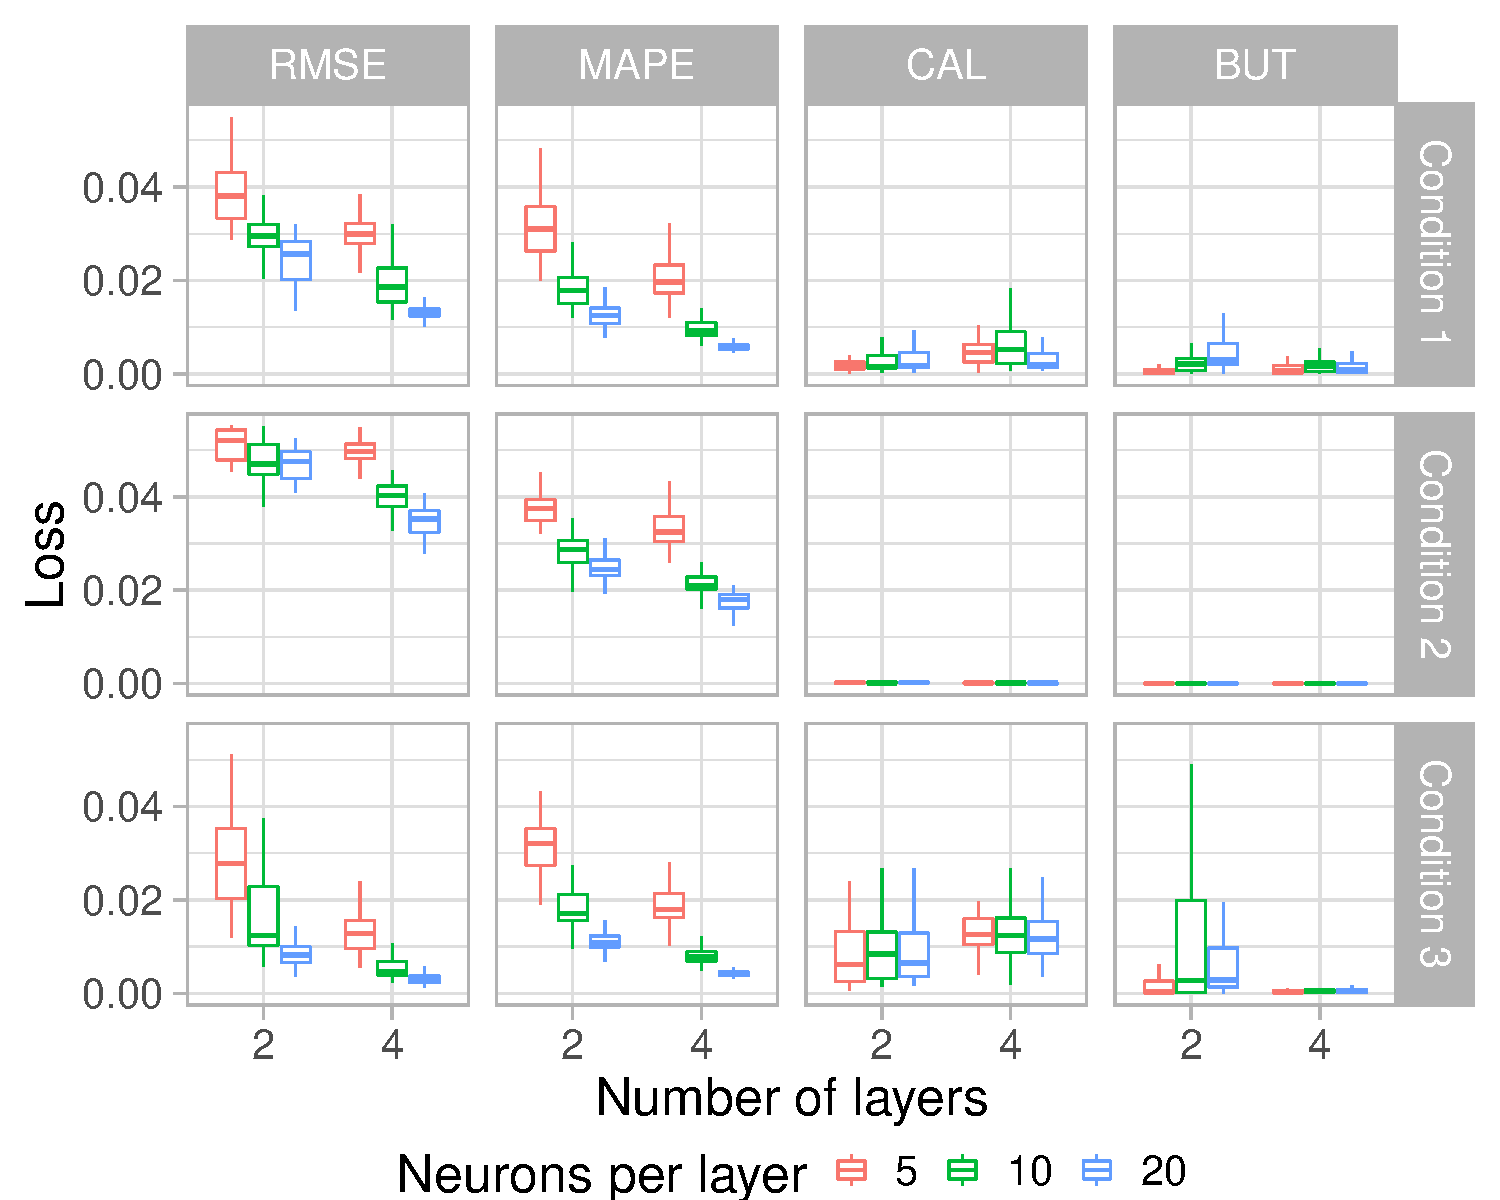
\includegraphics[width=0.6\textwidth]{figures/numexp_convergence_loss_bates.pdf}
\caption{Losses for different combination of number of layers and neurons per layer. Synthetic data is generated from the Bates model.\label{fig:conv_loss}}
%\end{wrapfigure}
\end{figure}

\begin{figure}
%\begin{wrapfigure}{r}{0.6\textwidth}
\centering
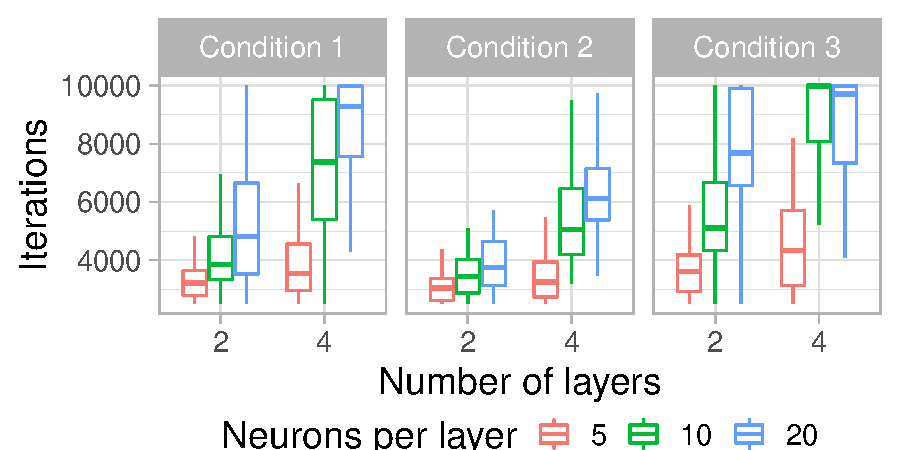
\includegraphics[width=0.6\textwidth]{figures/numexp_convergence_iter_bates.pdf}
\caption{Number of iterations before the calibration stops for different combination of number of layers and neurons per layer. Synthetic data is generated from the Bates model.\label{fig:conv_iter}}
%\end{wrapfigure}
\end{figure}

\textbf{Smoothing behaviors.}
A major challenge is the extrapolation of the implied volatility surface to unobserved data points.
Flexible non-parametric methods typically fail as they lack the guidance of a parametric model.
In \Cref{fig:smoothing} we calibrate ANN models with different loss terms and parameters initialization on a subsample of 100 options with narrow moneyness on the synthetic Bates data. 
The three models fit the train set almost perfectly.
Yet, we see that the ANN without arbitrage losses, $\lambda_1=\lambda_2=0$, fails extrapolate in a nonsensical way.
On the other hand the arbitrage-free model with $\lambda_1=\lambda_2=10$ behaves very smoothly.
The last model is initialized with the weights of an ANN model fitted to a Bates model itself fitted on the train set, see Appendix~B.3.
It is furthermore penalized so that its weights remain close to its initialization weights with $\lambda_3=1$.
This confirms that a regularized learning can produce an extrapolation mimicking the Bates model, with most notable differences in this example for the positive log-moneynesses.


\begin{figure}
  \centering
  \input{figures/smoothing}
  \vspace{-0.8cm}
\caption{Extrapolation with different loss specification and weights initialization.\label{fig:smoothing}}
\end{figure}




%% no time
%%\textbf{Soft versus hard constraints.}



